\documentclass[cn]{elegantbook}
\usepackage[square,numbers,sort&compress]{natbib}
\newcommand{\upcite}[1]{\textsuperscript{\textsuperscript{\cite{#1}}}}
\usepackage{diagbox}
\usepackage{algorithm}
\usepackage{algorithmicx}
\usepackage{algpseudocode}
\renewcommand{\algorithmicrequire}{\textbf{输入:}}
\renewcommand{\algorithmicensure}{\textbf{输出:}}

\tikzstyle{startstop} = [rectangle, rounded corners, minimum width = 2cm, minimum height=1cm,text centered, draw = black, fill = red!40]
\tikzstyle{arrow} = [->,>=stealth]

% title info
\title{模式识别作业4}
\subtitle{分类问题}
% bio info
\author{罗雁天}
\institute{清华大学电子系}
\version{2018310742}
\date{\today}
\logo{logo.png}
\cover{cover.jpg}

\begin{document}

\maketitle
\tableofcontents
\mainmatter
\hypersetup{pageanchor=true}
% add preface chapter here if needed
\chapter{迭代修正求权向量法}
\section{问题描述}
\noindent 给定两组数据:
\begin{equation}
\begin{aligned}
\omega_1&=\{(1,1); (2,0); (2,1); (0,2); (1,3);\} \\
\omega_2&=\{(-1,2); (0,0); (-1,0); (-1,-1); (0,-2);\}
\end{aligned}
\end{equation}
求出其识别函数、识别界面以及绘制出识别界面将该训练样本的区分结果。

\section{算法描述}
\noindent 使用迭代修正求权向量法对此问题进行二分类,我们有如下算法Algorithm \ref{alg:iter}
\begin{algorithm}[htb]
	\caption{迭代修正求权向量法二分类}
	\label{alg:iter}
	\begin{algorithmic}[1]
		\Require $\omega_1, \omega_2, c$
		\Ensure 最终的权向量$W$
		\State 将$\omega_1, \omega_2$用扩展特征向量$X,Y$表示,即在每一个坐标点的第三维都添加1;
		\State 计算$Z=[X;-Y]$
		\State 初始化权向量$W_0$,并且置$k=0$
		\While {True}
		\If {$\forall z \in Z, W_k^T\cdot z>0$}
		\State break
		\Else
		\State 选出$W_k^T\cdot z\le0$的分量组成$Z'$
		\State 计算$Z''=mean(Z')$
		\State 迭代修正权向量$W_{k+1}=W_k+c\cdot Z''$
		\EndIf
		\EndWhile
		\State 输出$W=W_k$
	\end{algorithmic}
\end{algorithm}

\section{实验结果}
在此,我们尝试了两种初始化$W$的方法,并且对实验结果进行了对比。

\subsection{随机初始化$W$}
在本小节,我们使用Matlab中的$rand()$函数对$W$进行初始化,经过$k=8$次迭代完全将两类分开。最终得到的权向量为$[3.9857,0.9991,-0.0660]^T$,因此,分类界面的方程为:
\begin{equation}
W^T\cdot z=0\Rightarrow 3.9857x + 0.9991y - 0.0660=0
\end{equation}

对任意的数据$\mathbf{z}=[x,y]^T$,线性识别函数为:
\begin{equation}
f(\mathbf{z})=\left\{
\begin{array}{cc}
\mathbf{z}\in \omega_1 & if \quad 3.9857x + 0.9991y - 0.0660>0 \\
\mathbf{z}\in \omega_2 & if \quad 3.9857x + 0.9991y - 0.0660\le 0 \\
\end{array}
\right.
\end{equation}

分类界面绘制如图\ref{fig1}所示。
\begin{figure}[!h]
	\centering
	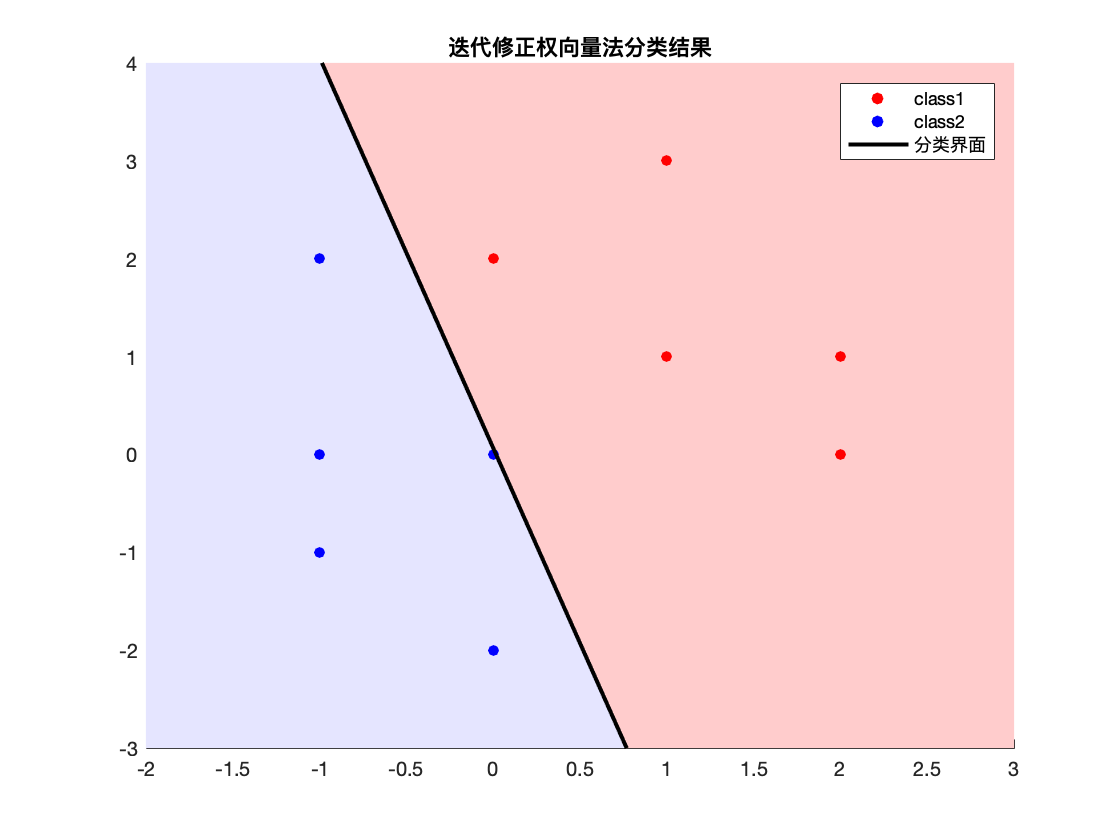
\includegraphics[width=\textwidth]{images/iterrand}
	\caption{\label{fig1}使用随机初始化$W$的方式进行迭代修正求权向量法二分类结果示意图}
\end{figure}

\subsection{全0初始化$W$}
在本小节,我们使用Matlab中的$zeros()$函数对$W$进行初始化,经过$k=4$次迭代完全将两类分开。最终得到的权向量为$[2.4,1.3,-1]^T$,因此,分类界面的方程为:
\begin{equation}
W^T\cdot z=0\Rightarrow 2.4x + 1.3y - 1=0
\end{equation}

对任意的数据$\mathbf{z}=[x,y]^T$,线性识别函数为:
\begin{equation}
f(\mathbf{z})=\left\{
\begin{array}{cc}
\mathbf{z}\in \omega_1 & if 2.4x + 1.3y - 1>0 \\
\mathbf{z}\in \omega_2 & if 2.4x + 1.3y - 1\le 0 \\
\end{array}
\right.
\end{equation}

分类界面绘制如图\ref{fig2}所示。
\begin{figure}[!h]
	\centering
	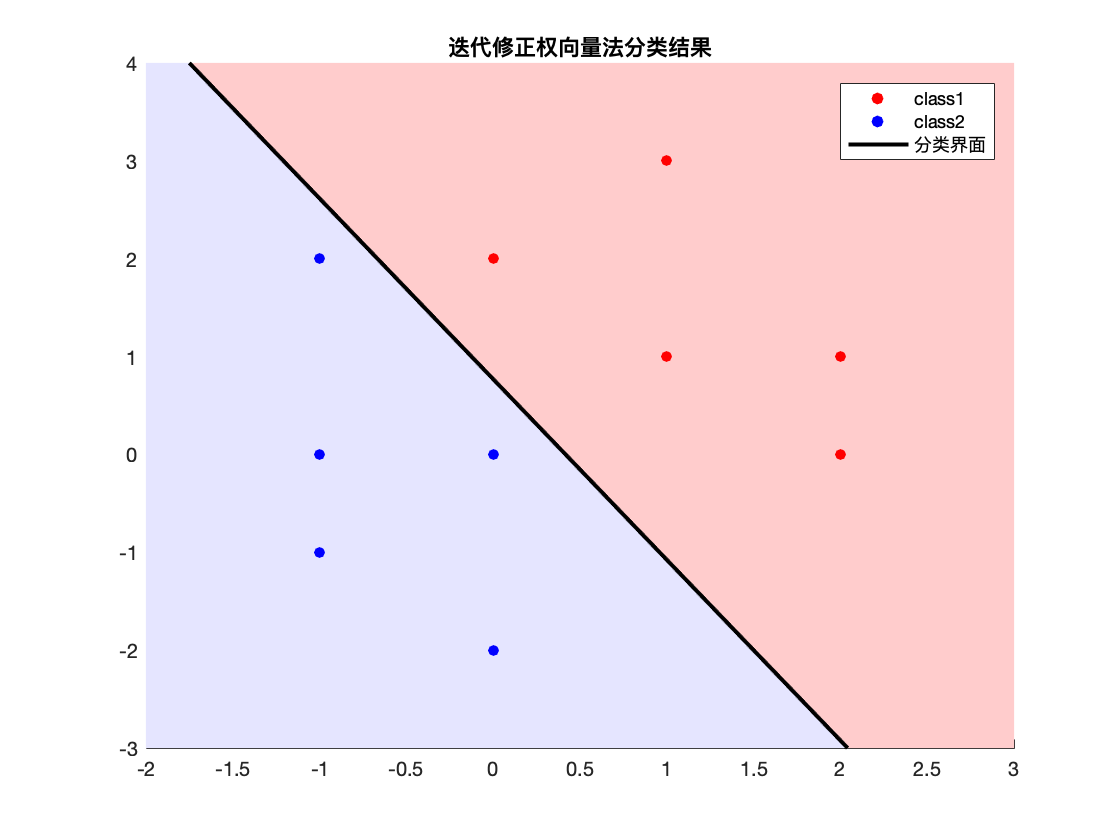
\includegraphics[width=\textwidth]{images/iterzeros}
	\caption{\label{fig2}使用全0初始化$W$的方式进行迭代修正求权向量法二分类结果示意图}
\end{figure}

\chapter{KNN}
\section{问题描述}
有两组二维数据,数据以txt文档的形式提供。对一个新的样本点,请尝试用KNN算法判断 它的所属组别。

\section{算法描述}
使用KNN算法对数据进行二分类的算法如Algorithm \ref{alg:knn}所示。

\begin{algorithm}[htb]
	\caption{KNN二分类}
	\label{alg:knn}
	\begin{algorithmic}[1]
		\Require 训练集($X,Y$),测试数据($z$)
		\Ensure 测试数据的类别
		\State 初始化k近邻的集合$knnlist$为前$k$个点,与k近邻距离的集合$distlist$为到前$k$个点的距离
		\For {$x\in X$}
		\State 计算距离最大的近邻为$maxk$,最大距离为$maxdist$
		\State 计算$x,z$之间的距离$dist$
		\If {$dist<maxdist$}
		\State 将$x$加入$knnlist$并将$maxk$在$knnlist$里删掉;
		\State 将$dist$加入$distlist$并将$maxdist$在$knnlist$里删掉;
		\EndIf
		\EndFor
		\State 统计$k$个最近邻样本中每个类别出现的次数
		\State 选择出现频率最大的类别作为未知样本的类别
	\end{algorithmic}
\end{algorithm}

\section{实验结果}
在实验中,我们选用不同的$k$来绘制不同的分类界面,并且对比其结果。

首先我们绘制出在$k=1,3,5,7$时的分类界面如图\ref{knnres}所示,从图中可以看出,当$k=1$时,算法转换为最近邻算法,训练集上的分类正确率为100\%,但是可以看出,分类界面非常不平滑,有点过拟合;当$k=3$时,可以看出相对于$k=1$的情况,分类结果依然正确率为100\%,但是分类界面比$k=1$的情况平滑了很多;当$k=5$时,可以看出,分类界面在进一步的平滑,但是分类的正确率已经不是$100\%$了;当$k=7$时,分类界面进一步平滑,但是分类的准确率也在进一步的降低。
\begin{figure}[!h]
	\centering
	\begin{minipage}[h]{0.48\linewidth}
		\centering
		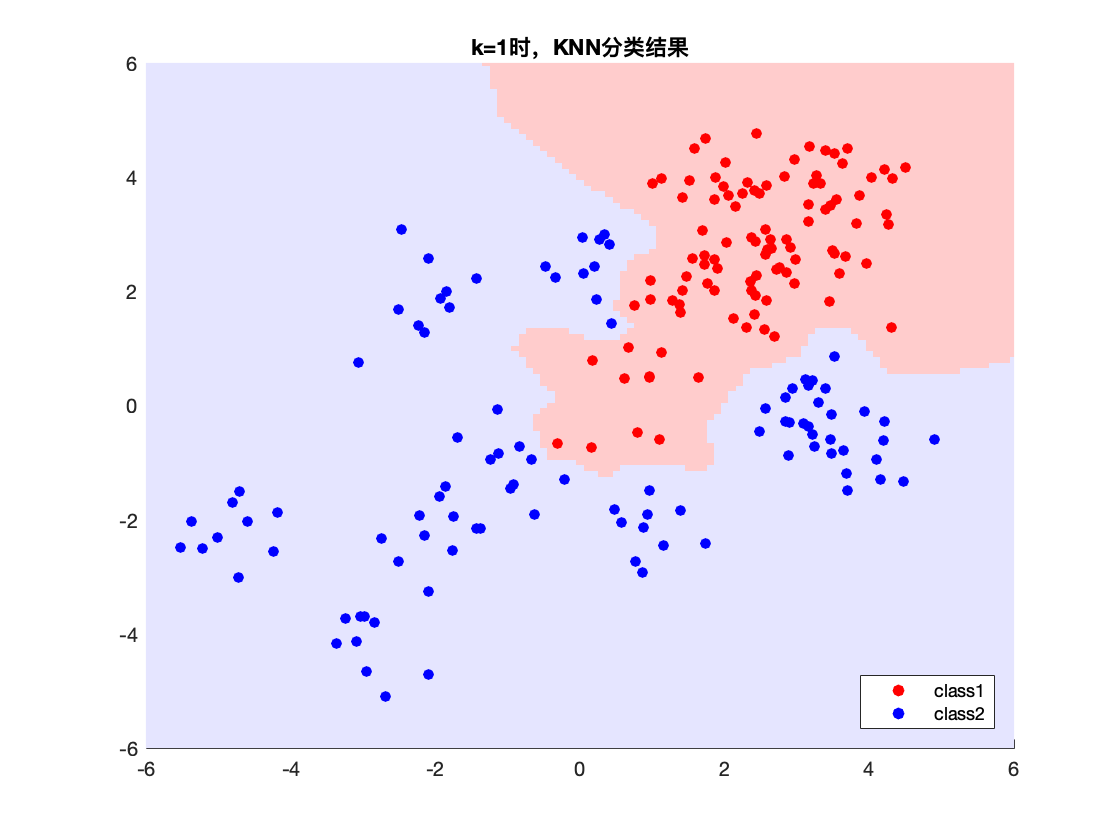
\includegraphics[width=\textwidth]{images/knnres1}
	\end{minipage}
\begin{minipage}[h]{0.48\linewidth}
	\centering
	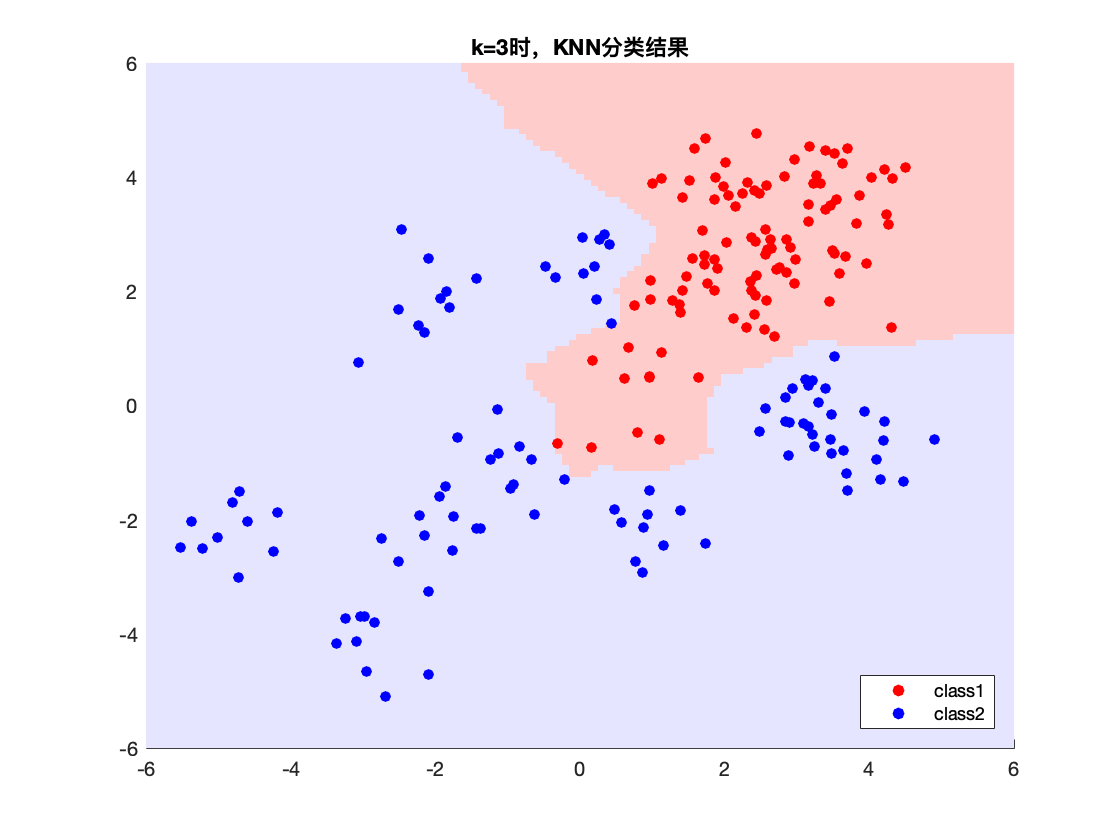
\includegraphics[width=\textwidth]{images/knnres2}
\end{minipage}
\begin{minipage}[h]{0.48\linewidth}
	\centering
	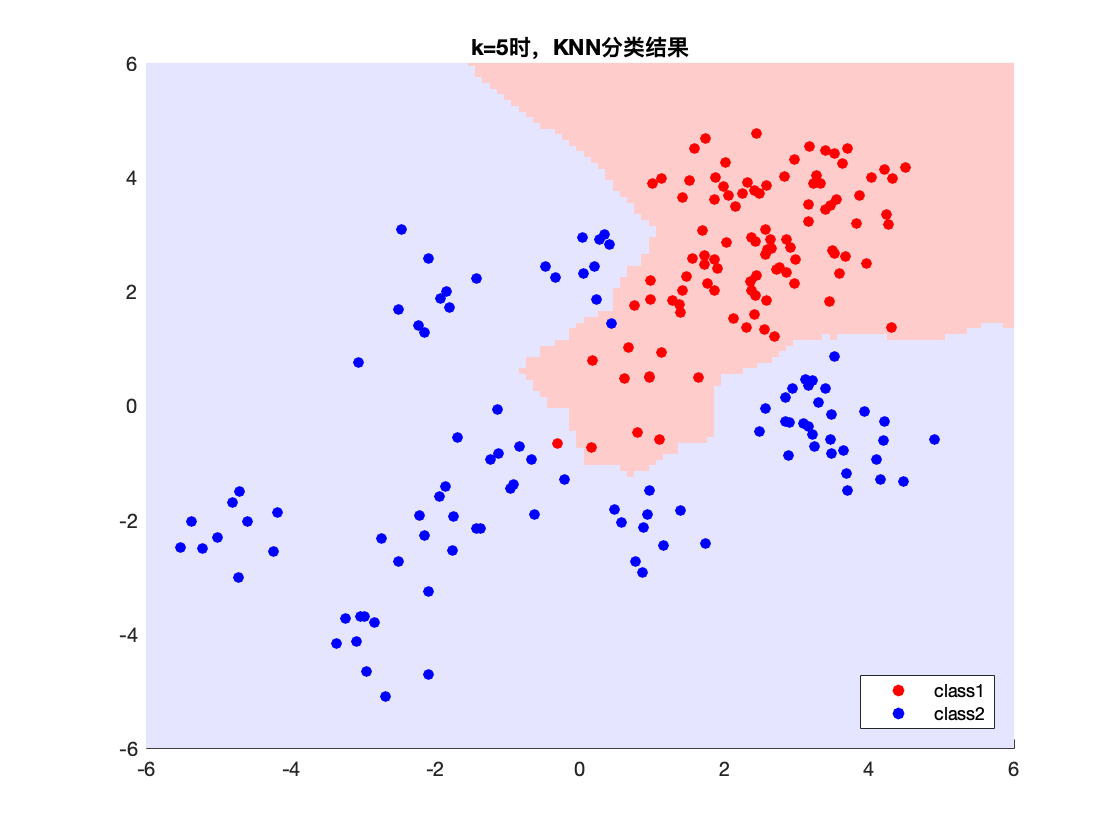
\includegraphics[width=\textwidth]{images/knnres3}
\end{minipage}
\begin{minipage}[h]{0.48\linewidth}
	\centering
	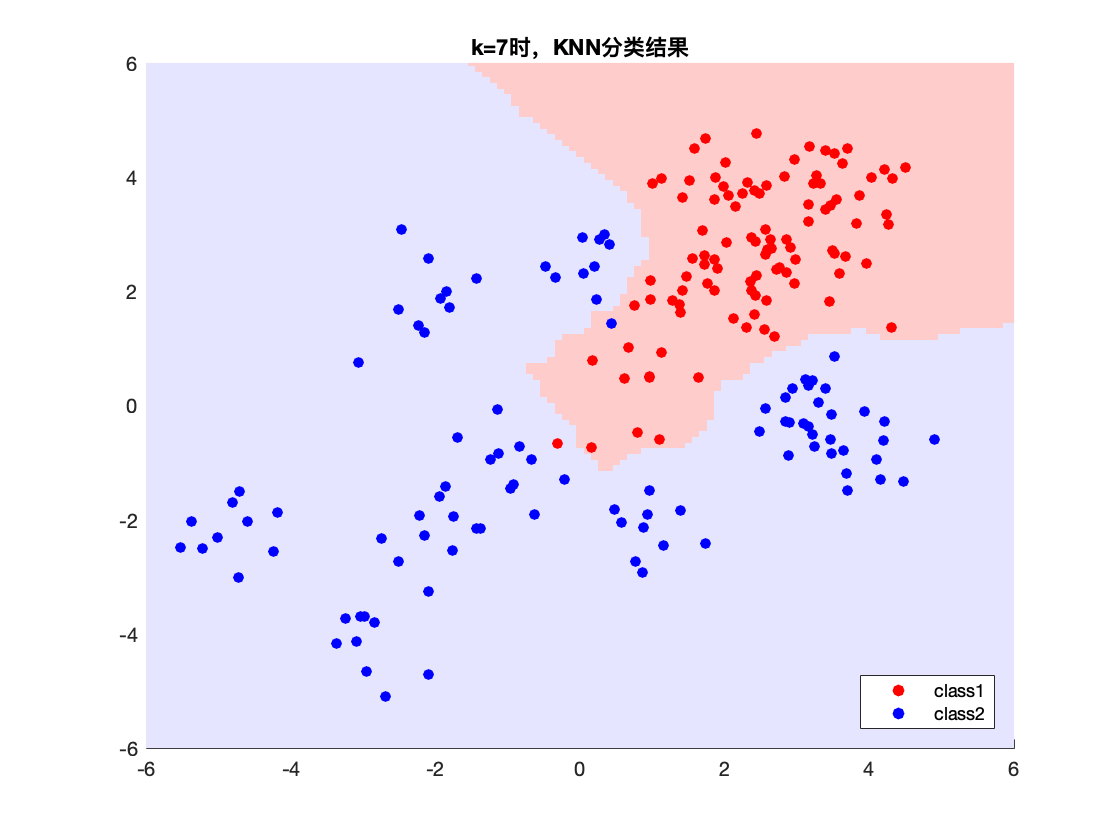
\includegraphics[width=\textwidth]{images/knnres4}
\end{minipage}
\caption{\label{knnres}$k=1,3,5,7$时,分类界面示意图}
\end{figure}

由此,我们可以推断出,随着$k$的增加,分类界面的平滑度会越来越高,但是训练集上分类的准确率也会越来越低,因此,我们取$k=1,3,5,\cdots,199$并计算每个$k$对应的准确率,绘制出正确率曲线如图\ref{fig3}所示,从曲线中我们可以清楚地看出正确率是随着$k$的增大而逐渐变小的。同时,我们绘制出$k=69$时的分类界面如图\ref{fig4}所示,从中可以看出,分类界面已经非常光滑了,但是训练集中分错的点也已经非常显而易见了。

\begin{figure}[!h]
	\centering
	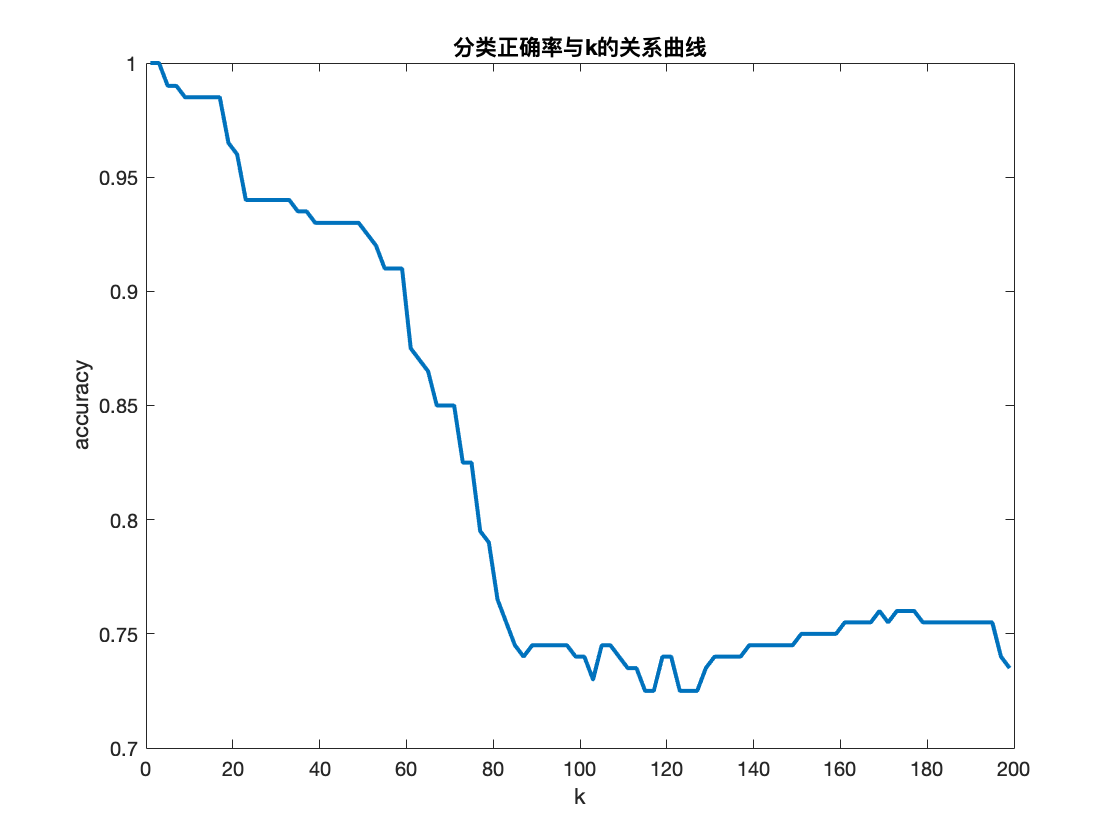
\includegraphics[width=\textwidth]{images/knnres5}
	\caption{\label{fig3}KNN分类正确率与近邻数k的关系曲线}
\end{figure}

\begin{figure}[!h]
	\centering
	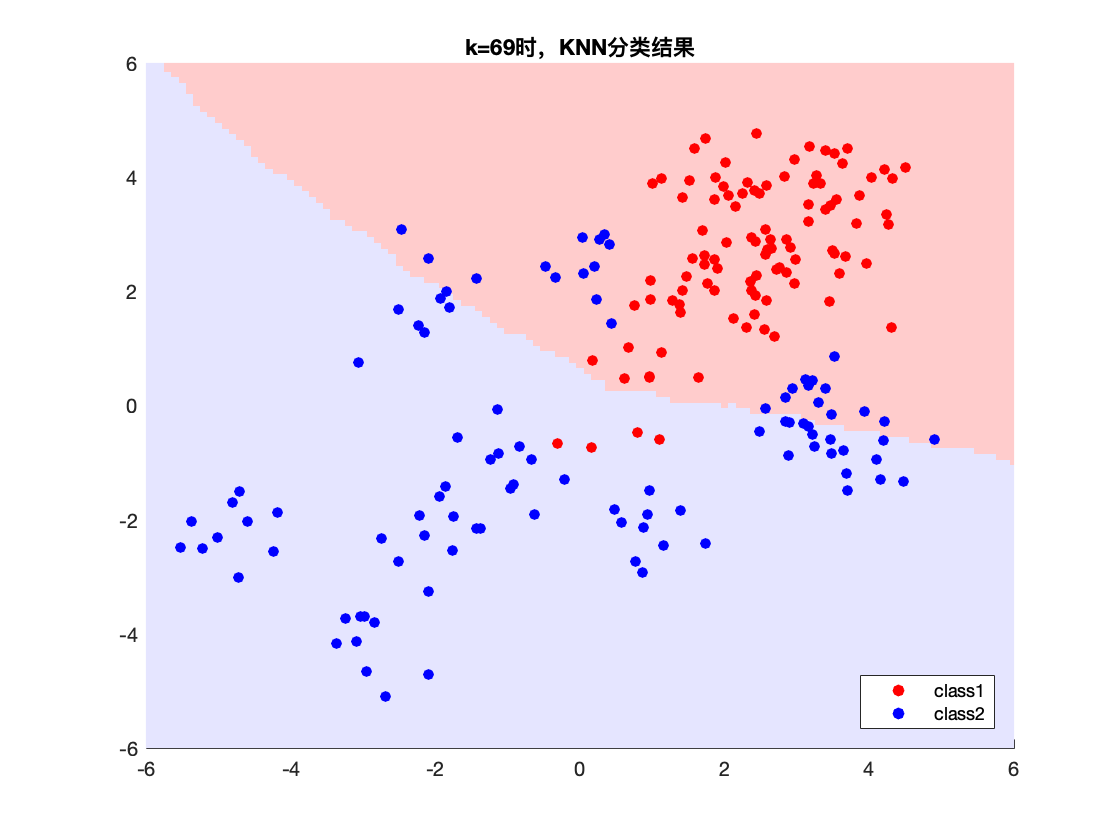
\includegraphics[width=\textwidth]{images/knnres6}
	\caption{\label{fig4}$k=69$时,分类界面示意图}
\end{figure}

\chapter{Fisher判别准则}
\section{问题描述}
\noindent 对下列两种情况,求采用Fisher判别准则 时的投影向量W和分类界面,并作图。
\begin{itemize}
	\item 情况1:
	\begin{equation}
	\begin{aligned}
	\omega_1&=\{(2,0); (2,2); (2,4); (3,3)\} \\
	\omega_2&=\{(0,3); (-2,2); (-1,-1); (1,-2); (3,-1)\}
	\end{aligned}
	\end{equation}
	\item 情况2:
	\begin{equation}
	\begin{aligned}
	\omega_1&=\{(1,1); (2,0); (2,1); (0,2); (1,3)\} \\
	\omega_2&=\{(-1,2); (0,0); (-1,0); (-1,-1); (0,-2)\}
	\end{aligned}
	\end{equation}
\end{itemize}

\section{算法描述}
Fisher判别准则本质上是找到一个投影平面,使得投影之后类内距离小、类间距离大。课件上已经给出了详细的公式推导,在此只给出相应的算法描述:

\begin{algorithm}[htb]
	\caption{Fisher判别准则进行二分类}
	\label{alg:fisher}
	\begin{algorithmic}[1]
		\Require 训练集($\omega_1,\omega_2$),测试数据$x$
		\Ensure 测试数据分类类别
		\State 计算两个类的类中心:$M_i=\frac{1}{N_i}\sum_{X\in \omega_i}X,\quad i=1,2$
		\State 计算各类类内离散度矩阵:$S_i=\sum_{X\in \omega_i}(X-M_i)(X-M_i)^T$
		\State 计算总类内离散度矩阵:$S_w=S_1+S_2$
		\State 计算类间离散度矩阵:$S_B=(M_1-M_2)(M_1-M_2)^T$
		\State 计算投影向量:$W_0=\frac{S_w^{-1}(M_1-M_2)}{\left||S_w^{-1}(M_1-M_2)|\right|}$
		\State 确定分类阈值点$y_0$
		\State 计算$y=W_0^Tx$
		\State 如果$y>y_0$,则$x\in\omega_1$,否则,$x\in\omega_2$
	\end{algorithmic}
\end{algorithm}

\section{实验结果}
实验中,我们按照如下两种方式确定阈值点$y_0$:
\begin{equation}
\begin{aligned}
y_0^{(1)}&=\frac{\tilde{m_1}+\tilde{m_2}}{2}=\frac{W_0^T(M_1+M_2)}{2} \\
y_0^{(2)}&=\frac{N_1\tilde{m_1}+N_2\tilde{m_2}}{N_1+N_2}=\frac{W_0^T(N_1M_1+N_1M_2)}{N_1+N_2}
\end{aligned}
\end{equation}
\subsection{情况1}
此种情况下,使用$y_0^{(1)}=1.6965$作为阈值点时,我们可以得到最终的权向量为$W_0=[0.8357,0.5492]^T$,因此,分类界面的方程为:
\begin{equation}
W^T\cdot z=y_0\Rightarrow 0.8357x + 0.5492y - 1.6965=0
\end{equation}

对任意的数据$\mathbf{z}=[x,y]^T$,线性识别函数为:
\begin{equation}
f(\mathbf{z})=\left\{
\begin{array}{cc}
\mathbf{z}\in \omega_1 & if \quad 0.8357x + 0.5492y - 1.6965>0 \\
\mathbf{z}\in \omega_2 & if \quad 0.8357x + 0.5492y - 1.6965\le 0 \\
\end{array}
\right.
\end{equation}

绘制出分类界面示意图如图\ref{fig5}所示。


\begin{figure}[!h]
	\centering
	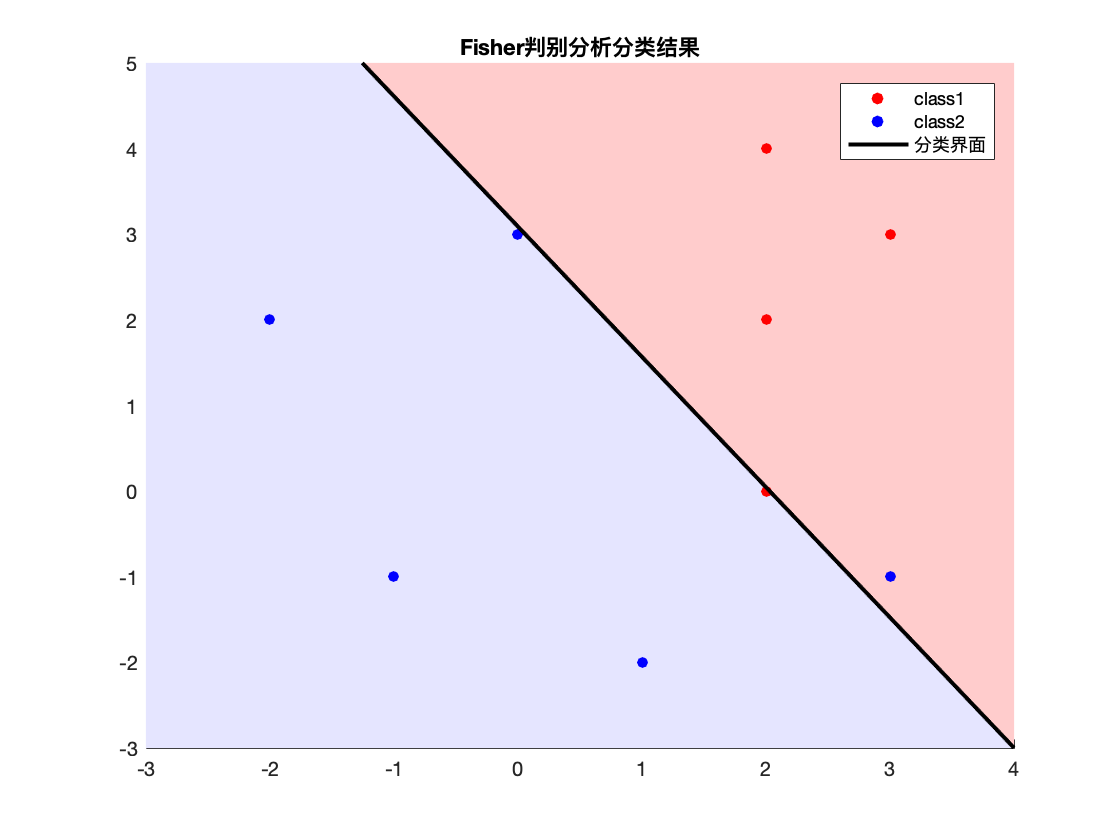
\includegraphics[width=\textwidth]{images/fisher1res1}
	\caption{\label{fig5}使用Fisher判别分析对情况1中数据进行分类的结果(阈值采用$y_0^{(1)})$}
\end{figure}

当采用$y_0^{(2)}=1.5388$作为阈值点时,我们可以得到最终的权向量为$W_0=[0.8357,0.5492]^T$,因此,分类界面的方程为:
\begin{equation}
W^T\cdot z=y_0\Rightarrow 0.8357x + 0.5492y - 1.5388=0
\end{equation}

对任意的数据$\mathbf{z}=[x,y]^T$,线性识别函数为:
\begin{equation}
f(\mathbf{z})=\left\{
\begin{array}{cc}
\mathbf{z}\in \omega_1 & if \quad 0.8357x + 0.5492y - 1.5388>0 \\
\mathbf{z}\in \omega_2 & if \quad 0.8357x + 0.5492y - 1.5388\le 0 \\
\end{array}
\right.
\end{equation}

绘制出分类界面示意图如图\ref{fig6}所示。

对比两种情况可以发现,对训练集数据分类的正确率并没有达到100\%,这是由于此问题在二维空间是线性不可分的,使用Fisher判别准则仅仅是使得类内距离小,类间距离大,并没有保证完全将其分开。并且,使用两种判别阈值的结果差别不大。


\begin{figure}[!h]
	\centering
	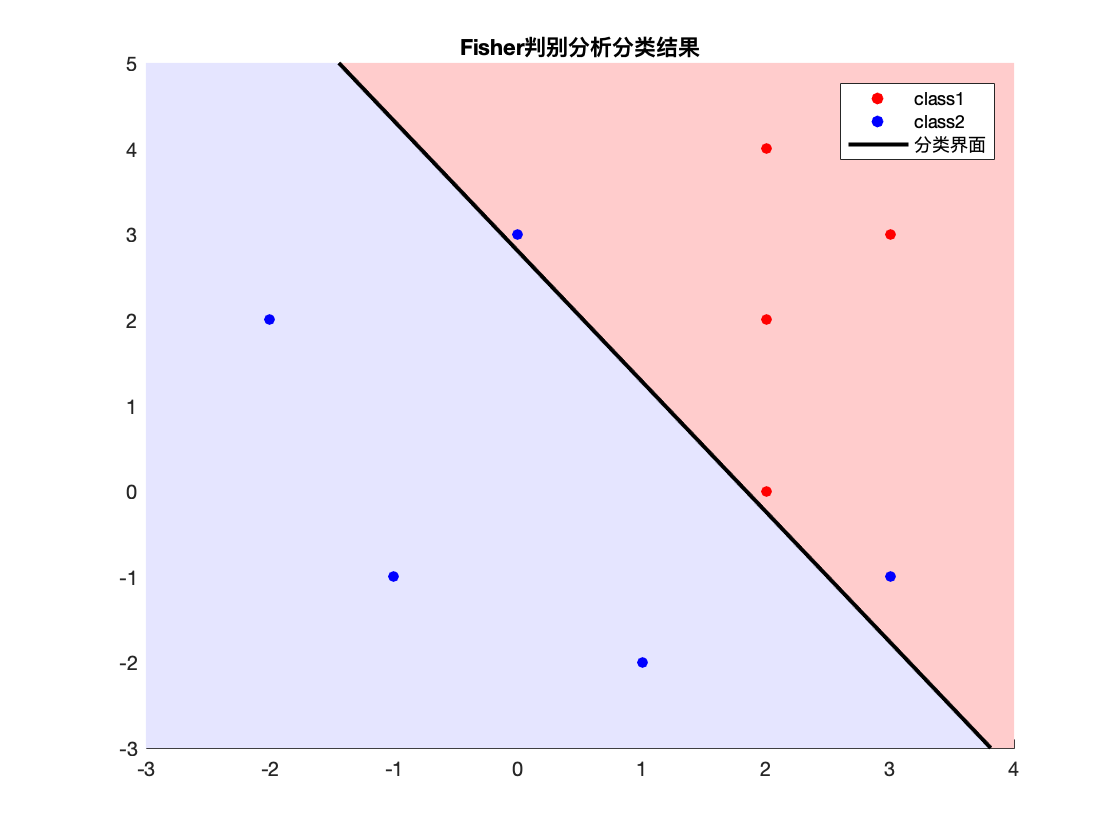
\includegraphics[width=\textwidth]{images/fisher1res2}
	\caption{\label{fig6}使用Fisher判别分析对情况1中数据进行分类的结果(阈值采用$y_0^{(2)})$}
\end{figure}

\subsection{情况2}
由于情况2中正负样本数是一致的,因此$y_0^{(1)}=y_0^{(2)}$,所以在此只进行了一次实验。得到最终的权向量为$W_0=[0.9185,0.3953]^T$,阈值$y_0=0.5128$因此,分类界面的方程为:
\begin{equation}
W^T\cdot z=y_0\Rightarrow 0.9185x + 0.3953y - 0.5128=0
\end{equation}

对任意的数据$\mathbf{z}=[x,y]^T$,线性识别函数为:
\begin{equation}
f(\mathbf{z})=\left\{
\begin{array}{cc}
\mathbf{z}\in \omega_1 & if \quad 0.9185x + 0.3953y - 0.5128>0 \\
\mathbf{z}\in \omega_2 & if \quad 0.9185x + 0.3953y - 0.5128\le 0 \\
\end{array}
\right.
\end{equation}

绘制出分类界面示意图如图\ref{fig7}所示。

\begin{figure}[!h]
	\centering
	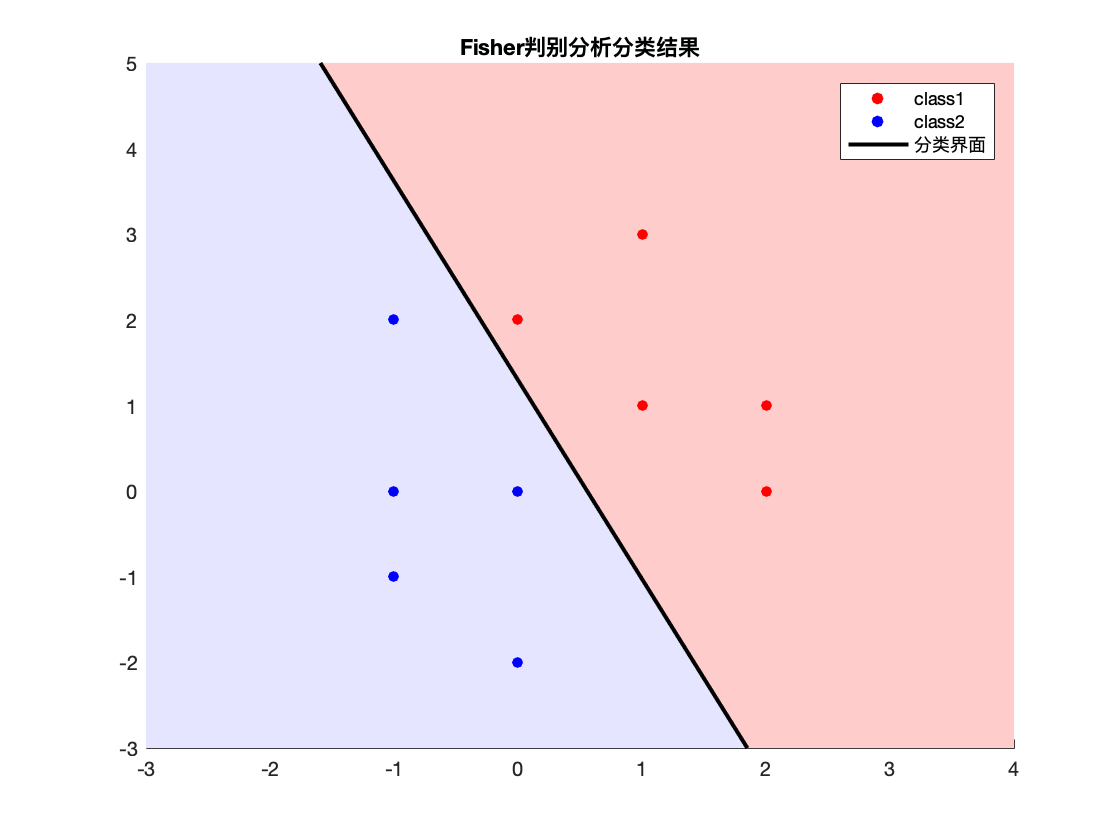
\includegraphics[width=\textwidth]{images/fisher2res1}
	\caption{\label{fig7}使用Fisher判别分析对情况2中数据进行分类的结果}
\end{figure}

由于此问题是线性可分的问题,因此可以得到较好的分类界面,训练数据的分类正确率也达到了100\%,与第一章中迭代修正求权向量的方法相比,此种方法对权向量的初始值不敏感,分类界面直观上也比随机初始化权向量的迭代修正求权向量的方法好。

\chapter{反思与总结}
至此,我们已经学过的二分类算法有最小欧式距离分类、迭代修正权向量法分类、Fisher判别准则分类,在此,我们使用如下数据:
\begin{equation}
\begin{aligned}
\omega_1&=\{(1,1); (2,0); (2,1); (0,2); (1,3)\} \\
\omega_2&=\{(-1,2); (0,0); (-1,0); (-1,-1); (0,-2)\}
\end{aligned}
\end{equation}
将三种算法的结果与SVM分类的结果进行对比如图\ref{compare}所示,从直观上来看,对于此数据集来说,使用0初始化的迭代修正权向量法、Fisher判别分析法和SVM分类的效果均比最小欧式距离分类的效果好。
\begin{figure}[!h]
	\centering
	\begin{minipage}[h]{0.48\linewidth}
		\centering
		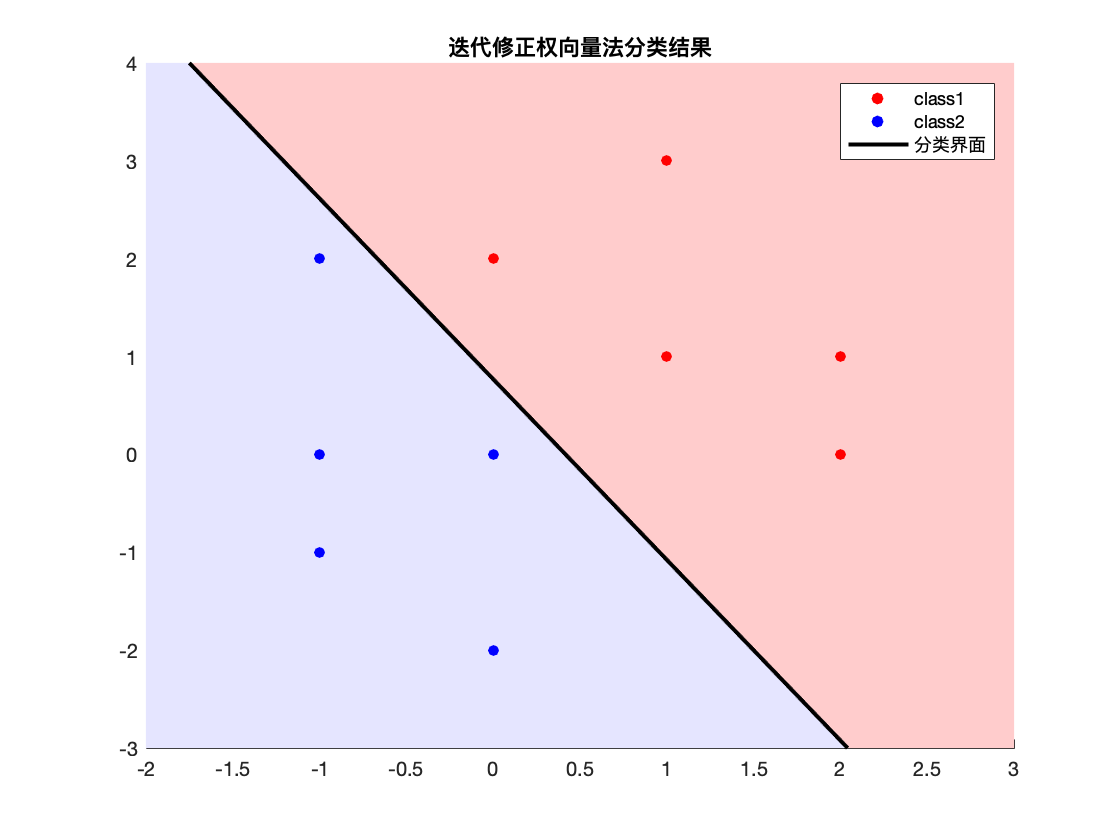
\includegraphics[width=\textwidth]{images/iterzeros}
	\end{minipage}
	\begin{minipage}[h]{0.48\linewidth}
		\centering
		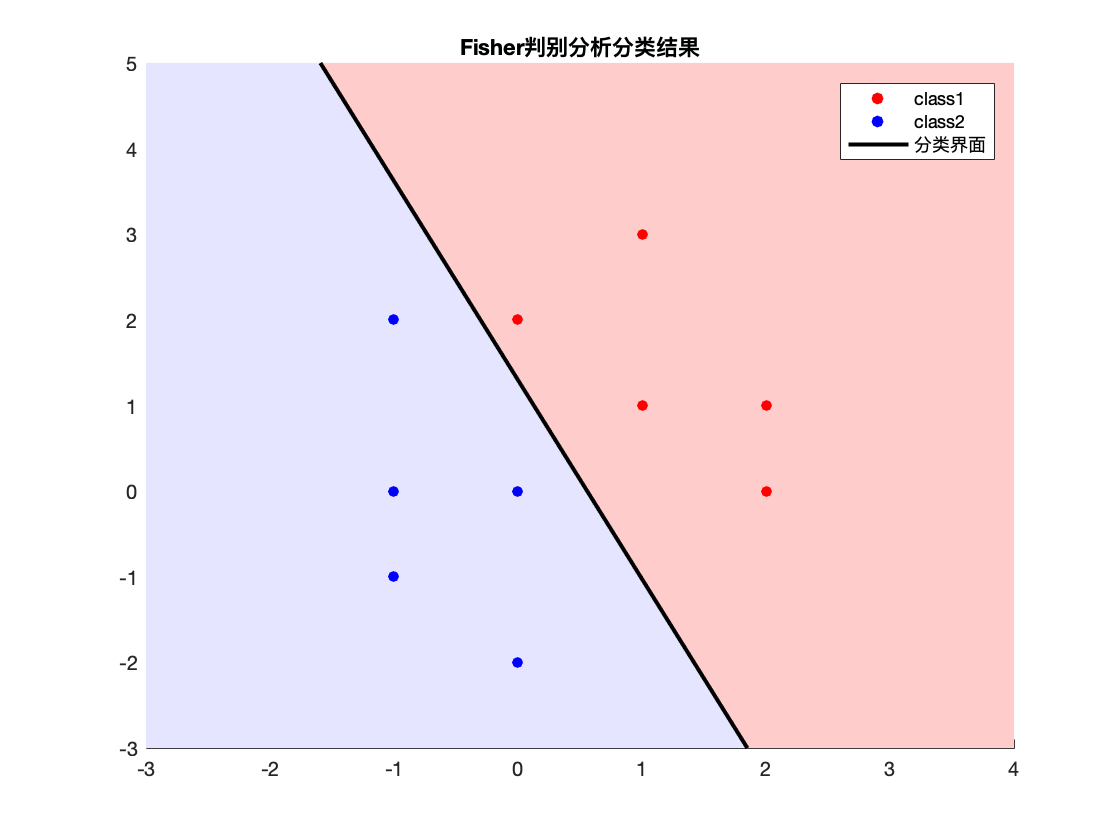
\includegraphics[width=\textwidth]{images/fisher2res1}
	\end{minipage}
	\begin{minipage}[h]{0.48\linewidth}
		\centering
		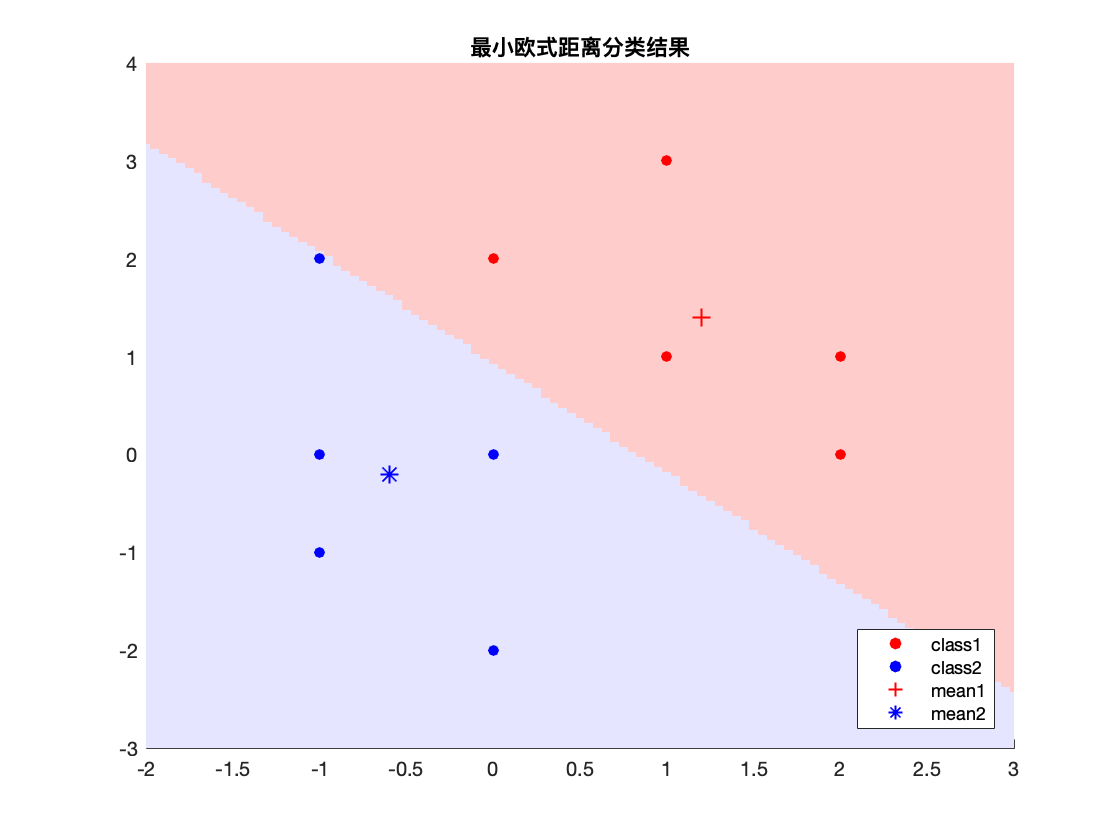
\includegraphics[width=\textwidth]{images/res}
	\end{minipage}
	\begin{minipage}[h]{0.48\linewidth}
		\centering
		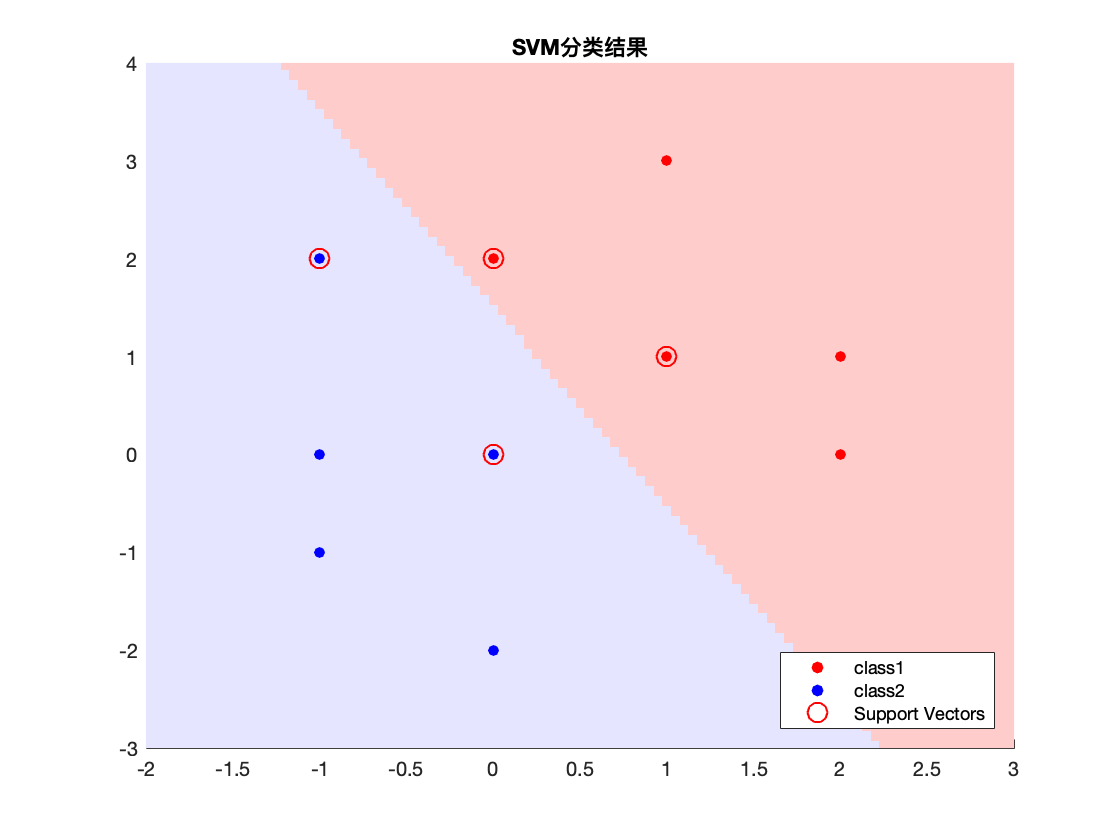
\includegraphics[width=\textwidth]{images/svmres}
	\end{minipage}
	\caption{\label{compare}四种二分类结果对比图}
\end{figure}


\chapter{代码说明}
\noindent 本次实验使用Matlab语言编写,所有代码放置在“code/”文件夹下:
\begin{itemize}
	\item iterative.m: 迭代修正求权向量法分类的主程序,直接执行便可以得到分类界面;
	\item knnclassify.m: KNN算法分类的主程序,直接执行便可以得到不同k下的分类界面以及正确率曲线;
	\item fishermain.m: Fisher判别分析算法分类的主程序,直接执行便可以得到情况1和情况2的分类界面图像;
	\item fisherclassify.m: 使用Fisher判别分析分类的函数,输入$\omega_1, \omega_2$,输出权向量$W_0$和分类阈值$y_0$,并且绘制分类界面图像。
	\item compare.m: 使用最小欧式距离分类和SVM分类的代码,直接执行绘制分类界面的图像。
\end{itemize}

\end{document}